\chapter{Social Engineering}
\label{chapter:se}

\section{Definition}

Nach einer groben Defintion des Wortes "Social Engineering" (engl. "soziale Manipulation")
handelt es sich um eine zwischenmenschliche Beeinflussung durch diverse psychologische
Tricks zwecksgemäß konkrete Verhaltensmuster hervorzurufen.
Social Engineering ist also ein Werkzeug, das nicht inhärent gut oder schlecht ist, sondern vielmehr durch seine Anwendung spezifiziert wird.


Geläufiger ist eine Definition im Sinne der Manipulation von Menschen, unrechtmäßig Informationen preiszugeben oder Aktionen auszuführen.
Unter derartige Aktionen fallen beispielsweise das Aushebeln von Sicherheitsfunktionen, das Tätigen von Überweisungen oder
das Installieren von Schadsoftware \bcite{1_enisa,2_bsi}.

Das Bundeskriminalamt legt in einer Forschungsstudie die offizielle Definition des Verfassungsschutzes Brandenburg
zugrunde: "Social Engineering ist der Versuch unter Ausnutzung menschlicher Eigenschaften Zugang zu Know-how zu erhalten.
Der Angreifer nutzt dabei Dankbarkeit, Hilfsbereitschaft, Stolz, Karrierestreben, Geltungssucht, Bequemlichkeit oder Konfliktvermeidung aus.
Dabei bieten häufig soziale Netzwerke oder auch Firmenwebseiten Möglichkeiten, um sich auf sein Opfer gründlich vorzubereiten.
Zu diesen 'Vorfeldermittlungen' können auch Anrufe im Unternehmen gehören.
Professionelle Angreifer versuchen dabei nicht, mit einem Anruf alle gewünschten Informationen zu erlangen,
dies könnte misstrauisch stimmen. Der Angerufene wird dabei im Gespräch nach vermeintlich nebensächlich erscheinenden Informationen gefragt."

In der Kurzfassung: Social Engineering ist eine zwischenmenschliche Manipulation,
bei der ein Unbefugter unter Vortäuschung falscher Tatsachen versucht, unberechtigten Zugang zu Informationen oder IT-Systemen zu erlangen \bcite{10_bka}.

In Bezug zu IT-Systemen und digitalen Daten wird Social Engineering auch konkreter als "Social Hacking" definiert \bcite{deficramer,defidgionos}.

\section{Angriffsvektoren}

\subsection{Methodik}

Obgleich unterschiedliche Social Engineering Angriffe fundamental verschieden ablaufen,
so haben sie dennoch eine grundlegende Struktur gemeinsam.
Diese Struktur lässt sich in vier Phasen einteilen:

\begin{minipage}{.5\linewidth}
    \begin{itemize}
        \setlength\itemsep{1em}
        \item 1) Research
        \item 2) Hook
        \item 3) Play
        \item 4) Out
    \end{itemize}
\end{minipage}
\hfill
\begin{minipage}{.5\linewidth}
    \centering
    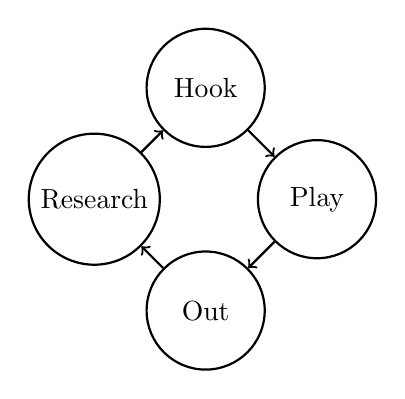
\begin{tikzpicture}[node distance={2cm}, thick, main/.style = {draw, circle, minimum size=15mm}]
        \node[main] (1) {Research};
        \node[main] (2) [above right of=1] {Hook};
        \node[main] (3) [below right of=2] {Play};
        \node[main] (4) [below right of=1] {Out};
        \draw[->] (1) -- (2);
        \draw[->] (2) -- (3);
        \draw[->] (3) -- (4);
        \draw[->] (4) -- (1);
    \end{tikzpicture}
\end{minipage}
\bcite{4_mdpi,cycle,ransomware}

\subsubsection{Research}
In der ersten Phase sucht der Angreifer sein Opfer aus und sammelt alle erwerblichen Informationen
im Zusammenhang mit dieser Person. Anhand dessen kann ein möglicher Angriffsvektor etabliert werden.
Der Erfolg eines Angriffes ist oft abhängig von ausführlicher Recherche, weshalb ein Großteil des zeitlichen
Aufwandes in dieser Phase steckt \bcite{4_mdpi,cycle,ransomware}.

\subsubsection{Hook}
In der "Hook" Phase baut der Angreifer eine Beziehung mit dem Opfer auf. Die Qualität dieser Beziehung bestimmt
die folgende Kooperation des Opfers. Abhängig von dem exakten Angriffsvektor kann diese Phase beispielsweise
eine langwierige Beziehung durch etwa Social Media darstellen. In anderen Angriffen definiert diese Phase den ersten
Eindruck im Affekt einer Situation, etwa durch freundliche Gestik oder Mimik. Es reichen für die meisten Menschen
bereits 100ms\footnote{Millisekunden} aus, um über Attraktivität, Sympathie, Vertrauenswürdigkeit, Kompetenz und
Aggressivität zu urteilen \bcite{firstimpression}, weshalb der erste Eindruck bei gewissen Social Engineering
Taktiken elementar ist \bcite{4_mdpi,cycle,ransomware}.

\subsubsection{Play}
In der dritten Phase nutzt der Angreifer die zuvor erlangten Informationen und die Beziehung zum Opfer aus,
um dieses dazu zu bewegen, sensible Daten preiszugeben, oder eine sicherheitskritische Aktion auszuführen \bcite{4_mdpi,cycle,ransomware}.

\subsubsection{Out}
Zuletzt zieht sich der Angreifer in der letzten Phase zurück, ohne jegliche Beweise eines Angriffes zurückzulassen.
Zum Beispiel werden digitale Fußabdrücke gelöscht, sodass der Angriff gegebenenfalls nicht auffällt,
die Identität des Angreifers anonym bleibt, und die Möglichkeit besteht, zukünftig erneut Kontakt aufzunehmen \bcite{4_mdpi,cycle,ransomware}.

\subsection{Klassifikation}

Social Engineering Angriffe können hinsichtlich verschiedener Aspekte klassifiziert werden\footnote{Social Engineering Angriffe können gegebenenfalls mehrere dieser Aspekte kombinieren.}.
Einerseits lassen sich verschiedene Angriffsvektoren nach dem verwendeten Medium unterscheiden.
Auf diese Weise lassen sich die folgenden zwei Kategorien identifizieren:

\begin{minipage}{.5\linewidth}
    \begin{itemize}
        \setlength\itemsep{1em}
        \item 1) menschlich
        \item 2) computerbasiert
    \end{itemize}
\end{minipage}
\hfill
\begin{minipage}{.5\linewidth}
    \centering
    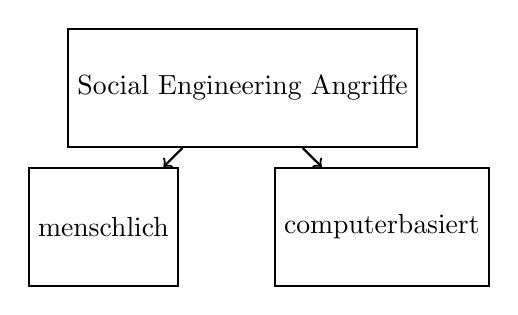
\begin{tikzpicture}[node distance={2.5cm}, thick, main/.style = {draw, rectangle, minimum size=15mm}]
        \node[main] (1) {Social Engineering Angriffe};
        \node[main] (2) [below left of=1] {menschlich};
        \node[main] (3) [below right of=1] {computerbasiert};
        \draw[->] (1) -- (2);
        \draw[->] (1) -- (3);
    \end{tikzpicture}
\end{minipage}
\bcite{1_enisa,4_mdpi}

Andererseits können Angriffsvektoren danach klassifiziert werden, wie die Angriffstechnik ausgeführt wird.
Somit entstehen die folgenden drei Klassifikationen:

\begin{minipage}{.5\linewidth}
    \begin{itemize}
        \setlength\itemsep{1em}
        \item 1) sozial
        \item 2) technisch
        \item 2) physisch
    \end{itemize}
\end{minipage}
\hfill
\begin{minipage}{.5\linewidth}
    \centering
    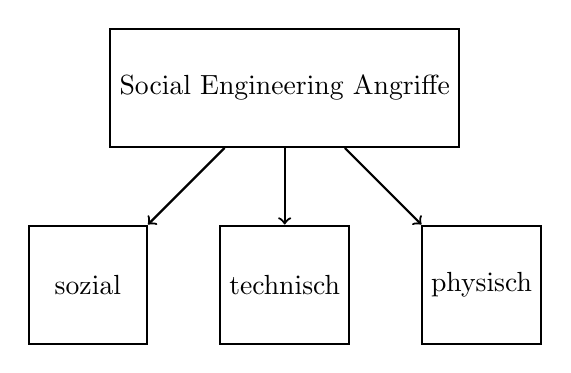
\begin{tikzpicture}[node distance={2.5cm}, thick, main/.style = {draw, rectangle, minimum size=15mm}]
        \node[main] (1) {Social Engineering Angriffe};
        \node[main] (3) [below of=1] {technisch};
        \node[main] (2) [left of=3] {sozial};
        \node[main] (4) [right of=3] {physisch};
        \draw[->] (1) -- (2);
        \draw[->] (1) -- (3);
        \draw[->] (1) -- (4);
    \end{tikzpicture}
\end{minipage}
\bcite{4_mdpi}

\subsubsection{menschliche Angriffe}

Im Falle von menschlichen Angriffen kommt es, durch persönlichen Kontakt, zu direkter Interaktion zwischen dem Angreifer und seinem Opfer.
Diese Angriffe können durchaus auch digital ablaufen, etwa über beliebige Messaging-Plattformen, und verwenden gezielte psychologische Manipulation,
die der Angreifer spezifisch auf sein Opfer abstimmt \bcite{4_mdpi, 1_enisa}.

\subsubsection{computerbasierte Angriffe}

Computerbasierte Angriffe, oder auch Softwarebasierte Angriffe, werden mithilfe von Computern\footnote{darunter zählen auch Smartphones oder anderweitige computerähnliche Geräte}
ausgeführt, um Informationen des Opfers zu sammeln. Diese Art von Angriff ist in der Lage eine Vielzahl
von potentiellen Opfern in kürzester Zeit zu erreichen \bcite{4_mdpi, 1_enisa}.

\subsubsection{technische Angriffe}

Technische Angriffe zielen darauf ab, Information, wie Passwörter oder Kreditkarteninformationen, zu erlangen. Sie werden ausgeführt über das Internet durch die sozialen Medien,
Webseiten oder anderweitigen online Diensten \bcite{4_mdpi,seofwnep}. "Die Kommunikation über digitale Kanäle wie E-Mail bietet ein besonders günstiges Umfeld für Social Engineering.
Während der Täter sein Gegenüber in einer realen Gesprächssituation über alle Sinne hinweg täuschen muss, hat er
es bei der technisch vermittelten Kommunikation deutlich einfacher"\bcite{2_bsi}.

\subsubsection{soziale Angriffe}

Bei sozialen Angriffen wird das psychologische Verhalten und die Emotionen des Opfers ausgenutzt. Diese Angriffe sind am gefährlichsten und in Relation zu ihrer Quantität am
erfolgreichsten, da sie menschlichte Interaktion beinhalten \bcite{4_mdpi}.

\subsubsection{physische Angriffe}

Physische Angriffe definieren diejenigen Aktionen, bei denen der Angreifer selbst materiellen Daten sammelt und nach Informationen sucht.
Beispielsweise durchsucht der Angreifer Mülleimer,
rekonstruiert zerstörte Dokumente oder begeht Diebstahl \bcite{4_mdpi}.



% "Social-based attacks are performed through relationships with the victims to play on their psychology and emotion. These attacks are
% the most dangerous and successful attacks as they involve human interactions"\cite{4_mdpi} -> baiting, spear fishing
% "Technical-based attacks are conducted through internet via social networks and online services websites and they gather desired
% information such as passwords, credit card details, and security questions"\cite{4_mdpi}
% "Physical-based attacks refer to physical actions performed by the attacker to collect information about the target. An example
% of such attacks is searching in dumpsters for valuable documents"\cite{4_mdpi}



\subsection{Techniken}

Es ist nahezu unmöglich einen vollständigen Überblich über alle existenten Angriffsvektoren im Bereich des Social Engineering
zu liefern. Wie zuvor in \autoref{chapter:einleitung} erwähnt sind diverse Social Engineering Techniken mit aktuellen ICT konstant im Wandel.
Etwaige Angriffsmethoden sind wie folgt:

"Pretexting
This technique involves the use of a pretext -  a false justification for a specific course of action - to gain
trust and trick the victim.
Example: the attacker claims to work for IT support and requests the target's password for maintenance purposes."\cite{1_enisa}

"Pretexting Attacks
Pretexting attacks consist of inventing fake and convincing scenarios in order to steal a victim’s personal information.
They are based on pretexts that make the victim believe and trust the attacker [27]. The attack is performed via phone calls,
emails, or physical media. Attackers use publishing information on phone books, public web pages, or conferences where collaborators
in the same field meet to carry out their attack. The pretext may be an offer to perform a service or to get a job,
asking about personal information, helping a friend to get access to something, or winning a lottery."\cite{4_mdpi}

"Baiting
Baiting involves luring the victim into performing a specific task by providing easy access to something the victim wants.
Example: a USB flash drive infected with a keylogger and labelled "My private pics" left on the victim's doorstep."\cite{1_enisa}

"Baiting Attacks
Baiting attacks, also called road apples, are phishing attacks that invite users to click on a link to get free stuff.
They act like trojan horses where the attack is performed by exploiting unsecured computer materials such as storage media
or USB drives containing malware in a coffee shop to be found by victims. When the victims plug the USB drive into their computers,
the drive acts like a real world trojan horse and attacks the computer. This attack performs malicious actions in the background
without being noticed by the victims.
In [7], the authors described a baiting attack named controller area network (CANDY) to be launched as a trojan horse in
the infotainment system of automotive systems. This attack impacts the security capabilities of the vehicle by manipulating the
communication between the driver and the vehicle. It is performed by recording the driver’s voice which lets the attacker remotely
access the victim’s vehicle via back door, collect information about the vehicle circulation, and control the operation of the vehicle."\cite{4_mdpi}

"Quid pro quo
Quid Pro Quo, "something for something" in Latin, involves a request for information in exchange for a compensation.
Example: the attacker asks the victim's password claiming to be a researcher doing an experiment, in exchange for money."\cite{1_enisa}

piggybacking:
"Tailgating
Tailgating is the act of following an authorised person into a restricted area or system.
Example: the attacker, dressed as an employee, carries a large box and convinces the victim, who is an authorised employee
entering at the same time, to open the door of the data-centre using the victim's RFID pass."\cite{1_enisa}

"Tailgating Attacks
Tailgating attacks, also called piggybacking or physical access, consist of accessing an area or building by following someone
who has the security clearance to that place. They allow attackers access unauthorized buildings. For example, attackers ask a
victim to hold the door open because they forgot their company’ ID card or RFID (radio-frequency identification) card. They can als
borrow a computer or cellphone to perform malicious activities such as installing malware software [14].
For instance, RFID cards attacks are one of the most used attacks to access forbidden spaces for malicious purposes. Due to their
wide utilization and low cost, RFID systems are considered as the most emerging technology used by companies to control the access to
their facilities. Despite their advantages, they have vulnerabilities that can be exploited to cause serious security issues to companies.
RFID attacks can be performed over several layers of the interconnection system model (ISO) [28]. For instance, at the physical layer, the
RFID devices and the physical interface are targeted to manipulate an RFID communication. These attacks can cause temporary or permanent damage
of the RFID cards. At the network layer level, the attacker manipulates the RFID network such as the communication between the RFID entities and
data exchange between these entities."\cite{4_mdpi}

"Reverse Social Engineering Attacks
Reverse social engineering attackers claim to solve a network’s problem. This involves three main steps: causing a problem such as crashing the network;
advertising that the attacker is the only person to fix that problem; solving the problem while getting the desired information and leaving without being detected"\cite{4_mdpi}

Pop-Up Windows
Pop-up window attacks refer to windows appearing on the victim’s screen informing the connection is lost [35]. The user reacts by re-entering the login information
which runs a malicious program already installed with the window appearance. This program remotely forwards back the login information to the attacker. For instance,
pop-ups can be alert messages showing up randomly for online advertising to lure the victim in clicking on that window. Pop-ups also can be fake messages alerting about
a virus detection in the victim’s computer. The pop up will prompt the victim to download and install the suggested anti-virus software to protect the computer. They can
also be fake alerts stating that the computer storage is full and that it needs to be scanned and cleaned to save more space [35]. The victim panics and reacts quickly in
order to fix the problem, which activates the malware software carried in the pop-up window."\cite{4_mdpi}

"Phone/Email Scams Attacks
For this type of attacks, the attacker contacts the victim via phone or email seeking specific information or promising a prize or free merchandise.
They aim at influencing the victim to break the security rules or to provide personal information. Moreover, cellphone-based attacks can be performed
via calls and via short messaging services (SMS) or text messages, which are known as SMSishing attacks [35]. SMSishing attacks consist of sending fraudulent
messages and texts via cell phones to victims to influence them. They are similar to phishing attacks but they are performed in different ways. The efficiency of
the SMSishing attacks resides in the fact that victims can carry their cellphones anywhere and anytime. A received text message can include a malware even if it was
sent from trusted and known transmitter. The malware works as a background process installing backdoors for attackers to have access to information such as contact list,
messages, personal email, photos, notes, applications, and calendar. The scammer can install a root kit to control the cellphone completely [20]."\cite{4_mdpi}

"Robocalls Attacks
Robocall attacks have recently emerged as massive calls coming from computers to targeted persons with known phone numbers. They target cellphones, residential,
and work phones. A robocall is a device or computer program that automatically dials a list of phone numbers to deliver prerecorded messages. It is mainly based on
voice over the internet protocol (VoIP) to ensure several VoIP functions such as interactive voice response and text to speech [36]. These calls can be about offering
or selling services or solving problems. Helping to solve tax problems is a very known example of attack that has risen in intensity in recent years. In general, when
a victim answers the call, the phone number is stored in the attacker’s database. Even after blocking these calls, attackers’ systems call from other numbers. Robocall
attacks have become a serious problem in the USA and other countries. The only way for people to stop these calls is by not answering unknown phone numbers."\cite{4_mdpi}

"51\% of social engineering attacks are phishing"\cite{3_barracuda}
"Microsoft is the most impersonated brand, used in 57\% of phishing attacks"\cite{3_barracuda}

"That leads to a frightening
finding: The median time for
users to fall for phishing emails
is less than 60 seconds. "\cite{verizon2024}

Phishing, Baiting, Pretexting, Tailgating, Ransomware, impersonating on help desk, diversion theft, dumpster diving,
shoulder surfing, quid pro quo, pup-up windows, robocalls, reverse social engineering, online social engineering, phone social engineering,
stealing important documents, fake software, pharming, SMSishing, Whitelisting following
ScareWare, Watering-Hole, honeytraps, whaling, smishing, quishing, tishing, vishing, wishing, pharming, snowshoeing, USB Drop


